% !TeX spellcheck = pl_PL
\chapter{Testy algorytmów}
%%%%%%%%%%%%%%%%%%%%%%%%%%%%%%%%%%%%%%%%%%%%%%%%%%%%%%%%%%%%%%%%%%%%%%%%%%%%%%%%%%%%%%%%%%%%%%%%%%%%%%%%%%%%%%%%%%%%%%%%%%%%%%%%%%%%%%%%%%%%%%%%%%%%%%%%%%%%%%%%%%%%%%%%%%%%%%%%%%%%%%%%%%%%%%%%%%%%%%%%%%%%%%%%%%%%%%%%%%%%%%%%%%%%
\section{Opis testowania za pomocą solwerów SAT}
%%%%%%%%%%%%%%%%%%%%%%%%%%%%%%%%%%%%%%%%%%%%%%%%%%%%%%%%%%%%%%%%%%%%%%%%%%%%%%%%%%%%%%%%%%%%%%%%%%%%%%%%%%%%%%%%%%%%%%%%%%%%%%%%%%%%%%%%%%%%%%%%%%%%%%%%%%%%%%%%%%%%%%%%%%%%%%%%%%%%%%%%%%%%%%%%%%%%%%%%%%%%%%%%%%%%%%%%%%%%%%%%%%%%


Do testów $NDB$ użyte zostały zChaff oraz WalkSAT -- najbardziej popularny solwer kompletny i niekompletny.
Wszystkie testy zostały przeprowadzone za pomocą aplikacji konsolowej napisanej w języku C++17 z wykorzystaniem
biblioteki \textit{boost} do wygenerowania opcji programu i ułatwienia operacji na napisach.

\begin{figure}[h]
    \includegraphics[width=15cm]{img/NDBGeneratorHelp.png}
    \centering
    \caption{Opcje aplikacji testującej}
    \label{img:NDBGenHelp}
\end{figure}

Przy wywołaniu programu użytkownik może ustawić szereg wartości dla każdego dostępnego parametru i wybrać pożądany algorytm oraz typ testu.
Aplikacja następnie generuję losową $NDB$ dla każdej kombinacji parametrów, przeprowadza test oraz zapisuje wynik do pliku w formacie csv.

Możliwe jest także wygenerowanie pliku Negatywnej Bazy Danych w formacie \textit{ndb} tj. plik tekstowy zawierający napisy
nad alfabetem $\{0,1,*\}$, lub \textit{dimacs} - domyślnym formacie wykorzystywanym przez solwery SAT.
\begin{lstlisting}[caption={Przykładowy plik formatu \textit{dimacs}\\Zawartość składa się z komentarzy (linie zaczynające się znakiem \enquote{c}), definicji problemu (linia zaczynająca się znakiem \enquote{p})
i klauzul logicznych.\\ W tym przypadku opisywany jest problem CNF o trzech zmiennych i dwóch klauzulach reprezentujący formułę $(\neg x_1 \lor \neg x_3) \land (\neg x_2 \lor x_3 \lor x_1) $.},captionpos=b]

c Przykładowy plik cnf
p cnf 3 2
-1 -3 0
-2 3 1 0 
\end{lstlisting}

Aplikacja jest zintegrowana z napisaną w języku C implementacją algorytmu WalkSAT przedstawioną przez Uniwersytet w Rochester \cite{walksat-implementation}
oraz implementacją zChaff w języku C++ udostępnioną przez Uniwersytet w Princeton \cite{zchaff-implementation}.

Oba programy posiadają interfejs wiersza poleceń i przyjmują pliki w formacie \textit{dimacs}. Z powodu potrzeby testowania
znacznej ilości automatycznie generowanych formuł aplikacja testowa wywołuje procedury rozwiązujące bezpośrednio z kodu.
W przypadku solwera zChaff wymagane było jedynie załączenie pliku nagłówkowego i zalinkowaniu zbudowanej biblioteki, jednak przy integrowaniu
solwera WalkSAT konieczna była minimalna modyfikacja plików źródłowych w celu umożliwienia wywołania głównej funkcji oraz zresetowania
stanu po próbie rozwiązania każdej formuły.

%%%%%%%%%%%%%%%%%%%%%%%%%%%%%%%%%%%%%%%%%%%%%%%%%%%%%%%%%%%%%%%%%%%%%%%%%%%%%%%%%%%%%%%%%%%%%%%%%%%%%%%%%%%%%%%%%%%%%%%%%%%%%%%%%%%%%%%%%%%%%%%%%%%%%%%%%%%%%%%%%%%%%%%%%%%%%%%%%%%%%%%%%%%%%%%%%%%%%%%%%%%%%%%%%%%%%%%%%%%%%%%%%%%%
\section{Testy metod weryfikujących poprawność rekordów pozytywnych}
%%%%%%%%%%%%%%%%%%%%%%%%%%%%%%%%%%%%%%%%%%%%%%%%%%%%%%%%%%%%%%%%%%%%%%%%%%%%%%%%%%%%%%%%%%%%%%%%%%%%%%%%%%%%%%%%%%%%%%%%%%%%%%%%%%%%%%%%%%%%%%%%%%%%%%%%%%%%%%%%%%%%%%%%%%%%%%%%%%%%%%%%%%%%%%%%%%%%%%%%%%%%%%%%%%%%%%%%%%%%%%%%%%%%

\label{sec:red-str-test}
Algorytmy generacji $NDB$ \textit{Q-Hidden} oraz \textit{K-Hidden} nie gwarantują pokrycia całego zbioru $U~-~DB$.
Konieczne jest użycie odpowiedniej sumy kontrolnej. Po znalezieniu rozwiązania porównywany jest sufiks rekordu o określonej
długości z wynikiem wykorzystanej funkcji na pozostałej części ciągu bitowego. Jeżeli wynik się zgadza wynik jest uznawany na należący
do $DB$.

Zostały przetestowane następujące funkcje sumy kontrolnej:

\begin{itemize}
    \item Bit parzystości (1 bit)
    \item CRC-8 (8 bitów)
    \item CRC-16 (16 bitów)
    \item CRC-32 (32 bity)
    \item MD5 (128 bitów)
\end{itemize}
%%%%%%%%%%%%%%%%%%%%%%%%%%%%%%%%%%%%%%%%%%%%%%%%%%%%%%%%%%%%%%%%%%%%%%%%%%%%%%%%%%%%%%%%%%%%%%%%%%%%%%%%%%%%%%%%%%%%%%%%%%%%%%%%%%%%%%%%%%%%%%%%%%%%%%%%%%%%%%%%%%%%%%%%%%%%%%%%%%%%%%%%%%%%%%%%%%%%%%%%%%%%%%%%%%%%%%%%%%%%%%%%%%%%
\subsection{Wpływ parametrów generacji na ilość niepożądanych ukrytych ciągów bitowych}
%%%%%%%%%%%%%%%%%%%%%%%%%%%%%%%%%%%%%%%%%%%%%%%%%%%%%%%%%%%%%%%%%%%%%%%%%%%%%%%%%%%%%%%%%%%%%%%%%%%%%%%%%%%%%%%%%%%%%%%%%%%%%%%%%%%%%%%%%%%%%%%%%%%%%%%%%%%%%%%%%%%%%%%%%%%%%%%%%%%%%%%%%%%%%%%%%%%%%%%%%%%%%%%%%%%%%%%%%%%%%%%%%%%%

Jak wynika z testów, których wyniki są umieszczone na wykresach \ref{chrt:no-checksum-q-r} i \ref{chrt:no-checksum-k-r}
ilość nadmiarowych napisów ukrytych maleje wykładniczo wraz z wzrostem parametru $r$. Dla ilości rekordów pięciokrotnie większej niż długość napisu
zachowują się jedynie pojedyncze niepożądane ciągi. 

\begin{figure}[!h]
    \centering
    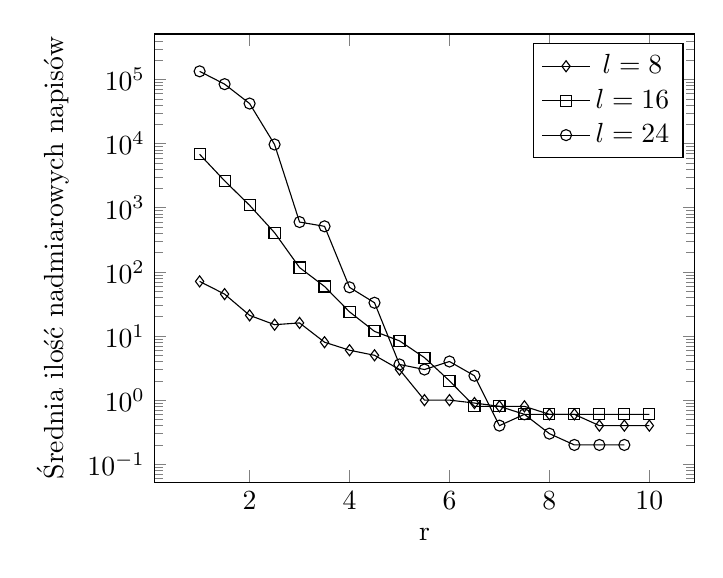
\begin{tikzpicture}
    \begin{semilogyaxis}[ylabel = {Średnia ilość nadmiarowych napisów}, xlabel={r}]
        \addplot[
    color=black,
    mark=diamond,
    ]
    coordinates {
        (10,0.4)(9.5,0.4)(9,0.4)(8.5,0.6)(8,0.6)(7.5,0.8)(7,0.8)(6.5,0.9)(6,1)(5.5,1)(5,3)(4.5,5)(4,6)(3.5,8)(3,16)(2.5,15)(2,21)(1.5,45)(1,71)
    };
    \addlegendentry{$l=8$}
        \addplot[
    color=black,
    mark=square,
    ]
    coordinates {
        (1,6823)(1.5,2631.6)(2,1092.4)(2.5,408.6)(3,116.8)(3.5,59.2)(4,23.8)(4.5,11.8)(5,8.4)(5.5,4.6)(6,2)(6.5,0.8)(7,0.8)(7.5,0.6)(8,0.6)(8.5,0.6)(9,0.6)(9.5,0.6)(10,0.6)
        
    };
    \addlegendentry{$l=16$}
    \addplot[
    color=black,
    mark=o,
    ]
    coordinates {
       (10,0)(9.5,0.2)(9,0.2)(8.5,0.2)(8,0.3)(7.5,0.6)(7,0.4)(6.5,2.4)(6,4)(5.5,3)(5,3.6)(4.5,33)(4,57.4)(3.5,513.4)(3,598.6)(2.5,9702)(2,42225)(1.5,84702)(1,134222)
               
    };
    \addlegendentry{$l=24$}
    
    
    \end{semilogyaxis}
    \end{tikzpicture}
    \caption{Zależność ilości nadmiarowych napisów od współczynnika ilości rekordów $r$~dla $NDB$
        wygenerowanych przez algorytm \textit{Q-Hidden} o parametrach $q~=~0.4$~i~$k~=~3$.}
    \label{chrt:no-checksum-q-r}
\end{figure}

\begin{figure}[!h]
    \centering
    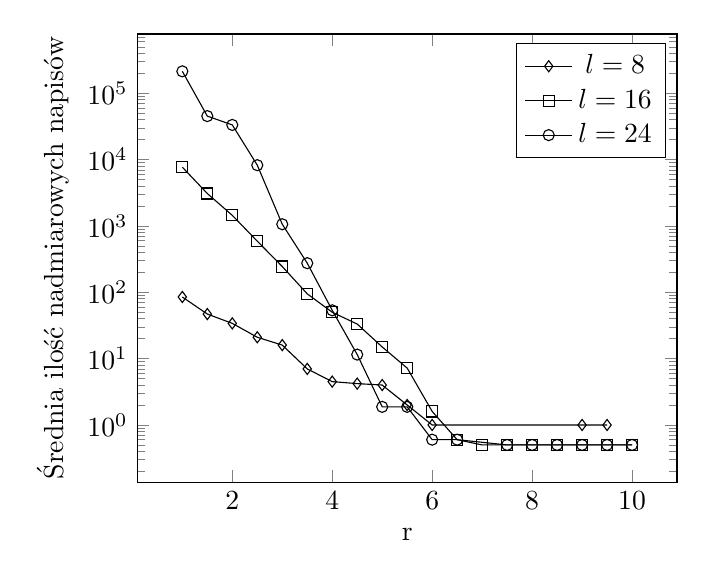
\begin{tikzpicture}    
    \begin{semilogyaxis}[ylabel = {Średnia ilość nadmiarowych napisów}, xlabel={r}]
    
    \addplot[
    color=black,
    mark=diamond,
    ]
    coordinates {
        (10,0)(9.5,1)(9,1)(8.5,0)(8,0)(7.5,0)(7,0)(6.5,0)(6,1)(5.5,2)(5,4)(4.5,4.2)(4,4.5)(3.5,7)(3,16)(2.5,21)(2,34)(1.5,47)(1,85)
    };
   \addlegendentry{$l=8$}
    
    \addplot[
    color=black,
    mark=square,
    ]
    coordinates {
        (1,7698.2)(1.5,3085.2)(2,1445.4)(2.5,589.8)(3,244.6)(3.5,94.8)(4,50)(4.5,33.2)(5,15)(5.5,7.2)(6,1.6)(6.5,0.6)(7,0.5)(7.5,0.5)(8,0.5)(8.5,0.5)(9,0.5)(9.5,0.5)(10,0.5)
        };
    \addlegendentry{$l=16$}
    
        \addplot[
    color=black,
    mark=o,
    ]
    coordinates {
        (1,214402)(1.5,45321)(2,33367)(2.5,8249)(3,1061.875)(3.5,274.875)(4,53.5)(4.5,11.5)(5,1.875)(5.5,1.875)(6,0.6)(6.5,0.6)(7,0)(7.5,0.5)(8,0.5)(8.5,0.5)(9,0.5)(9.5,0.5)(10,0.5)        
    };
    \addlegendentry{$l=24$}
    
    \end{semilogyaxis}
    
    \end{tikzpicture}
    \caption{Zależność ilości nadmiarowych napisów od współczynnika ilości rekordów $r$~dla $NDB$ 
        wygenerowanych przez algorytm \textit{K-Hidden}  o parametrach $p~=~\{0.7, 0.2, 0.1\}$~i~$k~=~3$.}    
    \label{chrt:no-checksum-k-r}
\end{figure}

Długość rekordu także ma znaczny wpływ na ich ilość, zwłaszcza dla małych wartości $r$, jednak przeprowadzanie testów dla całego przedziału $r \in [1, 10]$ dla $l > 24$ jest niepraktyczne ze względu na złożoność obliczeniową. 


\begin{figure}[!h]
    \centering
    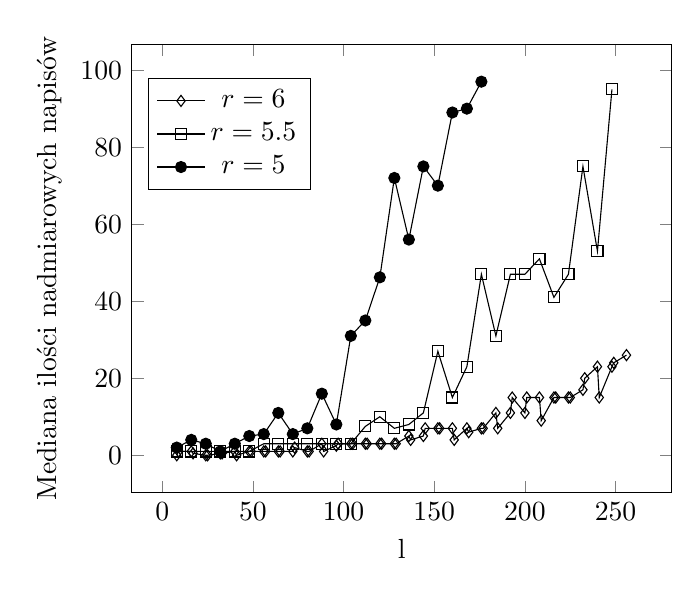
\begin{tikzpicture}
    \begin{axis}[ylabel = {Mediana ilości nadmiarowych napisów}, xlabel={l}, legend style={at={(0.03,0.8)},anchor=west}
    ]
    
    \addplot[
    color=black,
    mark=diamond,
    ]
    coordinates {
        (8,0.0)(9,1.0)(16,1.0)(17,0.5)(24,0.0)(25,0.0)(32,0.5)(33,0.5)(40,1.0)(41,0.0)(48,1.0)(49,1.0)(56,1.0)(57,1.0)(64,1.0)(65,1.0)(72,1.0)(73,2.0)(80,1.0)(81,1.0)(88,3.0)(89,1.0)(96,2.5)(97,3.0)(104,3.0)(105,3.0)(112,3.0)(113,3.0)(120,3.0)(121,3.0)(128,3.0)(129,3.0)(136,5.0)(137,4.0)(144,5.0)(145,7.0)(152,7.0)(153,7.0)(160,7.0)(161,4.0)(168,7.0)(169,6.0)(176,7.0)(177,7.0)(184,11.0)(185,7.0)(192,11.0)(193,15.0)(200,11.0)(201,15.0)(208,15.0)(209,9.0)(216,15.0)(217,15.0)(224,15.0)(225,15.0)(232,17.0)(233,20.0)(240,23.0)(241,15.0)(248,23.0)(249,24.0)(256,26.0)
        };
    \addlegendentry{$r=6$}
    \addplot[
    color=black,
    mark=square,
    ]
    coordinates {
       (8,1.0)(16,1.0)(24,1.0)(32,1.0)(40,1.0)(48,1.0)(56,3.0)(64,3.0)(72,3.0)(80,3.0)(88,3.0)(96,3.0)(104,3.0)(112,7.5)(120,10.0)(128,7.0)(136,8.0)(144,11.0)(152,27.0)(160,15.0)(168,23.0)(176,47.0)(184,31.0)(192,47.0)(200,47.0)(208,51.0)(216,41.0)(224,47.0)(232,75.0)(240,53.0)(248,95.0)        
    };
    \addlegendentry{$r=5.5$}
    \addplot[
    color=black,
    mark=*,
    ]
    coordinates {
       (8,2.0)(16,4.0)(24,3.0)(32,1.0)(40,3.0)(48,5.0)(56,5.5)(64,11.0)(72,5.5)(80,7.0)(88,16.0)(96,8.0)(104,31.0)(112,35)(120,46.2)(128,72)(136,56)(144,75)(152,70)(160,89)(168,90)(176,97)    
    };
    \addlegendentry{$r=5$}
    
    
    \end{axis}
    \end{tikzpicture}
    \caption{Zależność ilości nadmiarowych napisów od ilości rekordów $l$~dla $NDB$
        wygenerowanych przez algorytm \textit{Q-Hidden} o parametrach $q~=~0.3$~i~$k~=~3$.}
    \label{chrt:no-checksum-q-l}
\end{figure}

\begin{figure}[!h]
    \centering
    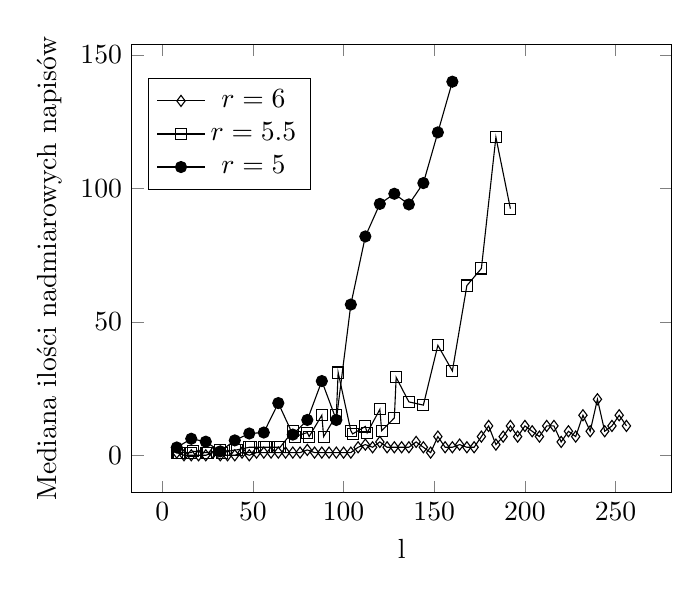
\begin{tikzpicture}
    \begin{axis}[ylabel = {Mediana ilości nadmiarowych napisów}, xlabel={l}, legend style={at={(0.03,0.8)},anchor=west}
    ]
    
    \addplot[
    color=black,
    mark=diamond,
    ]
    coordinates {
        (8,1)(12,0)(16,0)(20,0)(24,0)(28,1)(32,0)(36,0)(40,0)(44,1)(48,0)(52,1)(56,1)(60,1)(64,1)(68,1)(72,1)(76,1)(80,2)(84,1)(88,1)(92,1)(96,1)(100,1)(104,1)(108,3)(112,4)(116,3)(120,5)(124,3)(128,3)(132,3)(136,3)(140,5)(144,3)(148,1)(152,7)(156,3)(160,3)(164,4)(168,3)(172,3)(176,7)(180,11)(184,4)(188,7)(192,11)(196,7)(200,11)(204,9)(208,7)(212,11)(216,11)(220,5)(224,9)(228,7)(232,15)(236,9)(240,21)(244,9)(248,11)(252,15)(256,11)
    };
    \addlegendentry{$r=6$}
    \addplot[
    color=black,
    mark=square,
    ]
    coordinates {
(8,1.0)(9,1.0)(16,1.0)(17,1.5)(24,1.0)(25,1.0)(32,2.0)(33,1.0)(40,2.0)(41,2.0)(48,3.0)(49,3.0)(56,3.0)(57,3.0)(64,3.0)(65,3.0)(72,9.0)(73,7.0)(80,8.5)(81,7.0)(88,15.0)(89,7.0)(96,15.0)(97,31.0)(104,9.200000000000001)(105,8.0)(112,10.8)(113,8.4)(120,17.2)(121,9.200000000000001)(128,14.0)(129,29.200000000000003)(136,20.0)(144,18.8)(152,41.2)(160,31.6)(168,63.6)(176,70.0)(184,119.20000000000002)(192,92.4)

    };
    \addlegendentry{$r=5.5$}
    \addplot[
    color=black,
    mark=*,
    ]
    coordinates {
(8,2.9236581246446556)(16,6.193474588181687)(24,5.093895146368432)(32,1.4619326593310134)(40,5.576685112724268)(48,8.161785147204432)(56,8.521623408052468)(64,19.566637667041633)(72,7.7481427493677755)(80,13.238121928366919)(88,27.81180625303228)(96,13.222375917015809)(104,56.487992817647)(112,82)(120,94.2)(128,98)(136,94)(144,102)(152,121)(160,140)
    };
    \addlegendentry{$r=5$}
    \end{axis}
    \end{tikzpicture}
    \caption{Zależność ilości nadmiarowych napisów od ilości rekordów $l$~dla $NDB$
        wygenerowanych przez algorytm \textit{K-Hidden} o parametrach  $p~=~\{0.7, 0.2, 0.1\}$~i~$k~=~3$.}
    \label{chrt:no-checksum-k-l}
\end{figure}

Wraz ze wzrostem parametru $r$ zwiększa się wartość progowa długości rekordu, której przekroczenie powoduje znaczne zwiększenie tempa przyrostu ilości napisów nienależących do $DB$.
Jak wynika z wykresów \ref{chrt:no-checksum-q-l} i \ref{chrt:no-checksum-k-l} dla wartości $r=5$ pochodna funkcji wzrasta przy $l \approx 100$ a dla $r=5.5$ przy $l \approx 150$.

Z powodu znacznej fluktuacji wyników aby przedstawić dokładną tendencję konieczne było zastosowanie mediany zamiast wartości średniej. 

Negatywne Bazy Danych wygenerowane przez algorytm \textit{Q-Hidden} i \textit{K-Hidden} nie różnią się znacząco od siebie w kontekście tego testu.

%%%%%%%%%%%%%%%%%%%%%%%%%%%%%%%%%%%%%%%%%%%%%%%%%%%%%%%%%%%%%%%%%%%%%%%%%%%%%%%%%%%%%%%%%%%%%%%%%%%%%%%%%%%%%%%%%%%%%%%%%%%%%%%%%%%%%%%%%%%%%%%%%%%%%%%%%%%%%%%%%%%%%%%%%%%%%%%%%%%%%%%%%%%%%%%%%%%%%%%%%%%%%%%%%%%%%%%%%%%%%%%%%%%%
\subsection{Skuteczność funkcji sum kontrolnych}
%%%%%%%%%%%%%%%%%%%%%%%%%%%%%%%%%%%%%%%%%%%%%%%%%%%%%%%%%%%%%%%%%%%%%%%%%%%%%%%%%%%%%%%%%%%%%%%%%%%%%%%%%%%%%%%%%%%%%%%%%%%%%%%%%%%%%%%%%%%%%%%%%%%%%%%%%%%%%%%%%%%%%%%%%%%%%%%%%%%%%%%%%%%%%%%%%%%%%%%%%%%%%%%%%%%%%%%%%%%%%%%%%%%%
\begin{figure}[!h]
    \centering
    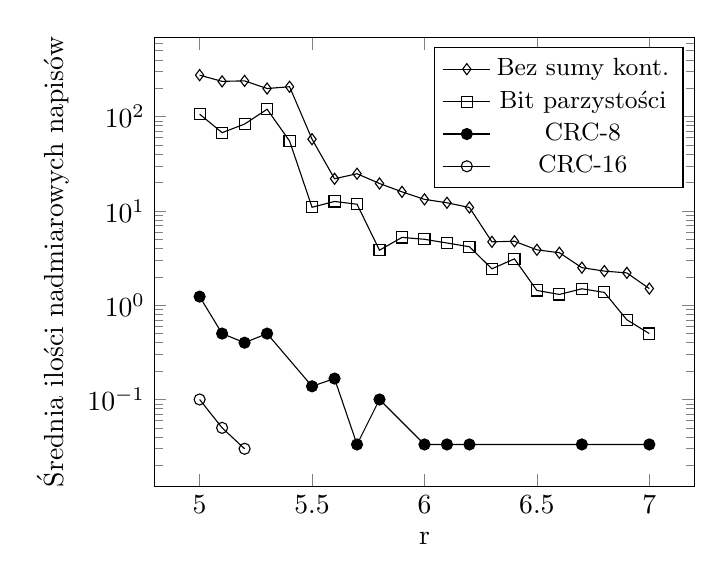
\begin{tikzpicture}
    \begin{semilogyaxis}[ylabel = {Średnia ilości nadmiarowych napisów}, xlabel={r}, legend style={font=\small}]
    
    
    \addplot[
    color=black,
    mark=diamond,
    ]
    coordinates {
        (5.0,275.17391304347825)(5.1,236.6)(5.2,239.5)(5.3,198.666666666666664)(5.4,207.53333333333333)(5.5,57.6)(5.6,21.933333333333334)(5.7,24.8)(5.8,19.533333333333335)(5.9,15.933333333333334)(6.0,13.266666666666667)(6.1,12.2)(6.2,10.866666666666667)(6.3,4.7)(6.4,4.7666666666666666)(6.5,3.86666666666667)(6.6,3.6)(6.7,2.5)(6.8,2.3)(6.9,2.2)(7.0,1.5)
    };
    \addlegendentry{Bez sumy kont.}
    \addplot[
    color=black,
    mark=square,
    ]
    coordinates {
       (5.0,106.34782608695652)(5.1,67.6)(5.2,83.35714285714286)(5.3,119.8)(5.4,55.13333333333333)(5.5,10.933333333333334)(5.6,12.6)(5.7,11.766666666666667)(5.8,3.8333333333333335)(5.9,5.233333333333333)(6.0,5)(6.1,4.566666666666667)(6.2,4.1666666666666667)(6.3,2.433333333333333)(6.4,3.1)(6.5,1.4333333333333333)(6.6,1.3)(6.7,1.49333333333333333)(6.8,1.3666666666666667)(6.9,0.7)(7.0,0.5)        
    };
    \addlegendentry{Bit parzystości}
    \addplot[
    color=black,
    mark=*,
    ]
    coordinates {
        (5.0,1.2333333333333334)(5.1,0.5)(5.2,0.4)(5.3,0.5)(5.4,0)(5.5,0.13793103448275862)(5.6,0.16666666666666666)(5.7,0.03333333333333333)(5.8,0.1)(5.9,0)(6.0,0.03333333333333333)(6.1,0.03333333333333333)(6.2,0.03333333333333333)(6.3,0)(6.4,0)(6.5,0)(6.6,0)(6.7,0.03333333333333333)(6.8,0)(6.9,0)(7.0,0.03333333333333333)
   };
    \addlegendentry{CRC-8}
    \addplot[
    color=black,
    mark=o,
    ]
    coordinates {
        (5.0,0.1)(5.1,0.05)(5.2,0.03)(5.3,0)(5.4,0)(5.5,0)(5.6,0)(5.7,0)(5.8,0)(5.9,0)(6.0,0)(6.1,0)(6.2,0)(6.3,0)(6.4,0)(6.5,0)(6.6,0)(6.7,0)(6.8,0)(6.9,0)(7.0,0)
    };
    \addlegendentry{CRC-16}
    
    \end{semilogyaxis}
    \end{tikzpicture}
    \caption{Zależność ilości nadmiarowych napisów od współczynnika ilości rekordów $r$~i~metody sumy kontrolnej.
        $NDB$ zostały wygenerowane przez algorytm \textit{K-Hidden} o parametrach  $p~=~\{0.7, 0.2, 0.1\}$~i~$k~=~3$ oraz \textit{Q-Hidden}
        o~parametrach $q=0.3$ i~$k=3$. Dla CRC-32 oraz MD5 nie zostały wykryte żadne nadmiarowe napisy.
    }
    \label{chrt:no-checksum-k-l}
\end{figure}

Wynik porównania różnych metod sumy kontrolnej pokrywa się z intuicją, według której każdy dodatkowy bit zmniejsza ilość ciągów bitowych
nienależących do $DB$ o połowę. Wynika z tego, że funkcja skrótu o długości 32 bitów, jest wystarczająca, żeby zapewnić spójność bazy danych
przy zastosowaniach w których nie trzeba przechowywać danych krytycznych.

W systemach uwierzytelniania zalecane jest jednak użycie większej wartości w celu zredukowania szansy konfliktu danych do praktycznie niemożliwej.  

%%%%%%%%%%%%%%%%%%%%%%%%%%%%%%%%%%%%%%%%%%%%%%%%%%%%%%%%%%%%%%%%%%%%%%%%%%%%%%%%%%%%%%%%%%%%%%%%%%%%%%%%%%%%%%%%%%%%%%%%%%%%%%%%%%%%%%%%%%%%%%%%%%%%%%%%%%%%%%%%%%%%%%%%%%%%%%%%%%%%%%%%%%%%%%%%%%%%%%%%%%%%%%%%%%%%%%%%%%%%%%%%%%%%
\section{Testy algorytmów generacji $NDB$}
%%%%%%%%%%%%%%%%%%%%%%%%%%%%%%%%%%%%%%%%%%%%%%%%%%%%%%%%%%%%%%%%%%%%%%%%%%%%%%%%%%%%%%%%%%%%%%%%%%%%%%%%%%%%%%%%%%%%%%%%%%%%%%%%%%%%%%%%%%%%%%%%%%%%%%%%%%%%%%%%%%%%%%%%%%%%%%%%%%%%%%%%%%%%%%%%%%%%%%%%%%%%%%%%%%%%%%%%%%%%%%%%%%%%
\subsection{Algorytm prefiksowy}
%%%%%%%%%%%%%%%%%%%%%%%%%%%%%%%%%%%%%%%%%%%%%%%%%%%%%%%%%%%%%%%%%%%%%%%%%%%%%%%%%%%%%%%%%%%%%%%%%%%%%%%%%%%%%%%%%%%%%%%%%%%%%%%%%%%%%%%%%%%%%%%%%%%%%%%%%%%%%%%%%%%%%%%%%%%%%%%%%%%%%%%%%%%%%%%%%%%%%%%%%%%%%%%%%%%%%%%%%%%%%%%%%%%%
\begin{figure}[!h]
    \centering
    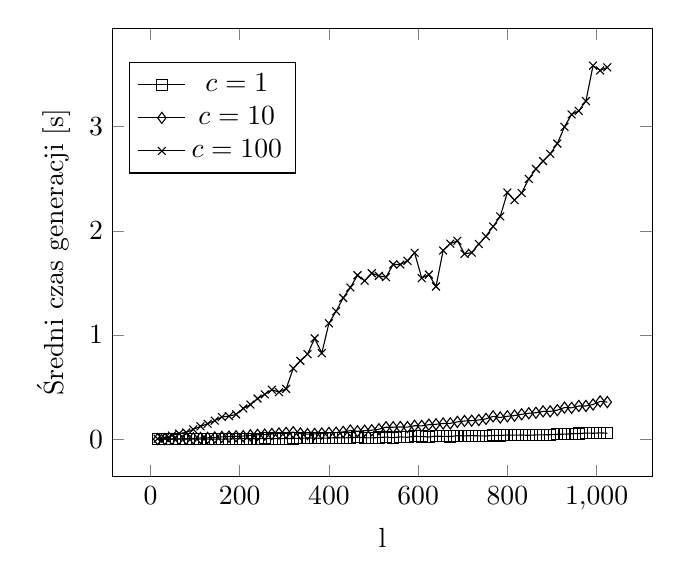
\begin{tikzpicture}
    \begin{axis}[ylabel={Średni czas generacji [s]}, xlabel={l}, legend style={at={(0.03,0.8)}, anchor=west}]
    \addplot[
    color=black,
    mark=square,
    ]
    coordinates {
        (16,0)(32,0)(48,0)(64,0)(80,0)(96,0)(112,0)(128,0.001)(144,0.001)(160,0.001)(176,0.001)(192,0.004)(208,0.005)(224,0.004)(240,0.005)(256,0.007)(272,0.006)(288,0.006)(304,0.006)(320,0.007)(336,0.008)(352,0.012)(368,0.01)(384,0.009)(400,0.011)(416,0.015)(432,0.012)(448,0.015)(464,0.018)(480,0.014)(496,0.012)(512,0.016)(528,0.02)(544,0.015)(560,0.022)(576,0.018)(592,0.028)(608,0.026)(624,0.021)(640,0.029)(656,0.027)(672,0.026)(688,0.033)(704,0.032)(720,0.034)(736,0.032)(752,0.031)(768,0.036)(784,0.036)(800,0.04)(816,0.039)(832,0.04)(848,0.037)(864,0.041)(880,0.042)(896,0.043)(912,0.047)(928,0.048)(944,0.052)(960,0.054)(976,0.059)(992,0.057)(1008,0.061)(1024,0.057)
    };
    \addlegendentry{$c = 1$}
    \addplot[
    color=black,
    mark=diamond,
    ]
    coordinates {
        (16,0)(32,0.001)(48,0.002)(64,0.003)(80,0.004)(96,0.008)(112,0.011)(128,0.013)(144,0.017)(160,0.022)(176,0.025)(192,0.028)(208,0.029)(224,0.037)(240,0.042)(256,0.044)(272,0.05)(288,0.055)(304,0.061)(320,0.067)(336,0.055)(352,0.049)(368,0.051)(384,0.055)(400,0.06)(416,0.063)(432,0.07)(448,0.083)(464,0.076)(480,0.082)(496,0.086)(512,0.096)(528,0.115)(544,0.115)(560,0.117)(576,0.116)(592,0.129)(608,0.128)(624,0.139)(640,0.143)(656,0.151)(672,0.152)(688,0.166)(704,0.175)(720,0.178)(736,0.184)(752,0.195)(768,0.219)(784,0.208)(800,0.22)(816,0.226)(832,0.239)(848,0.249)(864,0.254)(880,0.267)(896,0.267)(912,0.279)(928,0.303)(944,0.301)(960,0.319)(976,0.319)(992,0.333)(1008,0.363)(1024,0.356)
    };
    \addlegendentry{$c = 10$}
    \addplot[
    color=black,
    mark=x,
    ]
    coordinates{
(16,0.004)(32,0.012)(48,0.036)(64,0.054)(80,0.065)(96,0.094)(112,0.123)(128,0.148)(144,0.178)(160,0.213)(176,0.222)(192,0.238)(208,0.295)(224,0.332)(240,0.39)(256,0.43)(272,0.475)(288,0.452)(304,0.483)(320,0.68)(336,0.752)(352,0.816)(368,0.968)(384,0.826)(400,1.113)(416,1.228)(432,1.356)(448,1.456)(464,1.574)(480,1.521)(496,1.593)(512,1.568)(528,1.556)(544,1.678)(560,1.677)(576,1.713)(592,1.79)(608,1.547)(624,1.58)(640,1.466)(656,1.812)(672,1.877)(688,1.905)(704,1.779)(720,1.791)(736,1.874)(752,1.948)(768,2.042)(784,2.139)(800,2.368)(816,2.295)(832,2.364)(848,2.499)(864,2.595)(880,2.67)(896,2.739)(912,2.838)(928,2.999)(944,3.118)(960,3.152)(976,3.246)(992,3.587)(1008,3.54)(1024,3.57)
    };
     \addlegendentry{$c = 100$}
    \end{axis}
    \end{tikzpicture}
    \caption{Zależność czasu generacji $NDB$ za pomocą algorytmu prefiksowego od długości kodowanego ciągu.}
    \label{chrt:prefix-timegen}
\end{figure}

\begin{figure}[!h]
    \centering
    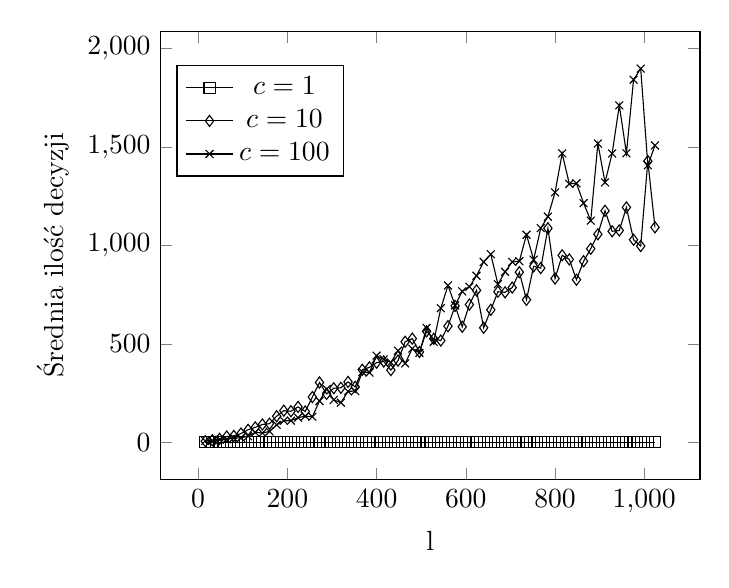
\begin{tikzpicture}
    \begin{axis}[ylabel={Średnia ilość decyzji}, xlabel={l}, legend style={at={(0.03,0.8)}, anchor=west}]
    \addplot[
    color=black,
    mark=square,
    ]
    coordinates {
        (16,1)(32,1)(48,1)(64,1)(80,1)(96,1)(112,1)(128,1)(144,1)(160,1)(176,1)(192,1)(208,1)(224,1)(240,1)(256,1)(272,1)(288,1)(304,1)(320,1)(336,1)(352,1)(368,1)(384,1)(400,1)(416,1)(432,1)(448,1)(464,1)(480,1)(496,1)(512,1)(528,1)(544,1)(560,1)(576,1)(592,1)(608,1)(624,1)(640,1)(656,1)(672,1)(688,1)(704,1)(720,1)(736,1)(752,1)(768,1)(784,1)(800,1)(816,1)(832,1)(848,1)(864,1)(880,1)(896,1)(912,1)(928,1)(944,1)(960,1)(976,1)(992,1)(1008,1)(1024,1)
    };
    \addlegendentry{$c = 1$}
    \addplot[
    color=black,
    mark=diamond,
    ]
    coordinates {
        (16,6)(32,11)(48,18)(64,30)(80,33)(96,45)(112,64)(128,76)(144,91)(160,95)(176,133)(192,161)(208,158)(224,180)(240,157)(256,230)(272,304)(288,246)(304,275)(320,277)(336,307)(352,282)(368,369)(384,381)(400,405)(416,411)(432,367)(448,415)(464,511)(480,527)(496,459)(512,564)(528,526)(544,517)(560,590)(576,693)(592,587)(608,700)(624,772)(640,582)(656,673)(672,765)(688,762)(704,786)(720,864)(736,724)(752,894)(768,885)(784,1087)(800,832)(816,950)(832,929)(848,826)(864,920)(880,983)(896,1057)(912,1176)(928,1072)(944,1076)(960,1193)(976,1029)(992,997)(1008,1428)(1024,1092)
    };
    \addlegendentry{$c = 10$}
    \addplot[
    color=black,
    mark=x,
    ]
    coordinates{
        (16,7.58)(32,9.62)(48,13.64)(64,15.66)(80,22.82)(96,23.46)(112,30.96)(128,50.46)(144,47.98)(160,55.4)(176,89.12)(192,109.92)(208,110.2)(224,125.62)(240,133.1)(256,130.02)(272,210.14)(288,271.48)(304,215.48)(320,201.76)(336,258.82)(352,260.8)(368,357.52)(384,354.78)(400,440.46)(416,421.7)(432,405.94)(448,465.48)(464,401.04)(480,476.28)(496,454.16)(512,581.14)(528,510.78)(544,681.64)(560,796.68)(576,695.76)(592,767.2)(608,789.98)(624,846.1)(640,916.52)(656,955.34)(672,803.06)(688,866.06)(704,916.28)(720,920.26)(736,1054.3)(752,927.76)(768,1087.86)(784,1146.14)(800,1269.42)(816,1467.4)(832,1312.3)(848,1315.68)(864,1214.8)(880,1125.92)(896,1517.3)(912,1319.9)(928,1467.12)(944,1711.14)(960,1468.12)(976,1841.54)(992,1898)(1008,1406.94)(1024,1507.66)
    };
    \addlegendentry{$c = 100$}
    \end{axis}
    \end{tikzpicture}
    \caption{Zależność liczby decyzji koniecznych do znalezienia pierwszego rozwiązania problemu przez solwer zChaff od długości ciągu i ilości rekordów dla $NDB$ wygenerowanej za pomocą algorytmu prefiksowego.}
    \label{chrt:prefix-dec}
\end{figure}

Algorytm prefiksowy jest bardzo prostą metodą generacji $NDB$, dlatego odwrócenie rezultatu jej działania nie stanowi problemu co zostało zaprezentowane w algorytmie \ref{alg:prefix-reverse}.

Generacja ma stosunkową niską złożoność czasową, nawet dla bardzo długich ciągów, jednak zawarcie wielu rekordów $DB$ może ją znacznie spowolnić\footnote{Testy czasowe algorytmów zostały przeprowadzone przez wyliczenie czasu procesora podczas działania określonej procedury na komputerze wyposażonym w procesor Intel i5-7200U 3.1 GHz i 16 GB pamięci RAM.}.
 
Kompletny solwer zChaff odwraca $NDB$ z jednym rekordem pozytywnym niemal natychmiast -- dla każdego przypadku została podjęta tylko jedna decyzja.
Przy zawarciu większej ilości napisów znalezienie jednego z nich staje się trudniejsze, jednak jest to nadal możliwe w czasie liniowym.

Natomiast dla solwera WalkSAT otrzymana struktura CNF jest problematyczna -- procedura degraduje się w kierunku losowego przeszukiwania o wykładniczej złożoności obliczeniowej.
Już dla stu napisów o długości 40 bitów metoda kończy działanie z powodu przekroczenia ustawionej na potrzeby testów wartości granicznej 10 prób po $10^9$ odwróceń przypisań.
\begin{figure}[!h]
    \centering
    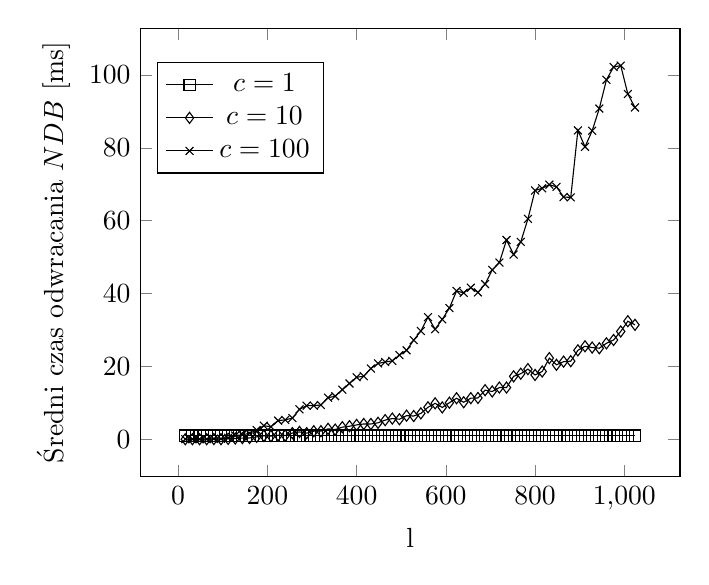
\begin{tikzpicture}
    \begin{axis}[ylabel={Średni czas odwracania $NDB$ [ms]}, xlabel={l}, legend style={at={(0.03,0.8)}, anchor=west}]
    \addplot[
    color=black,
    mark=square,
    ]
    coordinates {
        (16,1)(32,1)(48,1)(64,1)(80,1)(96,1)(112,1)(128,1)(144,1)(160,1)(176,1)(192,1)(208,1)(224,1)(240,1)(256,1)(272,1)(288,1)(304,1)(320,1)(336,1)(352,1)(368,1)(384,1)(400,1)(416,1)(432,1)(448,1)(464,1)(480,1)(496,1)(512,1)(528,1)(544,1)(560,1)(576,1)(592,1)(608,1)(624,1)(640,1)(656,1)(672,1)(688,1)(704,1)(720,1)(736,1)(752,1)(768,1)(784,1)(800,1)(816,1)(832,1)(848,1)(864,1)(880,1)(896,1)(912,1)(928,1)(944,1)(960,1)(976,1)(992,1)(1008,1)(1024,1)
    };
    \addlegendentry{$c = 1$}
    \addplot[
    color=black,
    mark=diamond,
    ]
    coordinates {
(16,0)(32,0)(48,0)(64,0)(80,0.04)(96,0.02)(112,0.1)(128,0.18)(144,0.3)(160,0.34)(176,0.64)(192,0.92)(208,0.86)(224,1.08)(240,1)(256,1.68)(272,2)(288,1.66)(304,2.2)(320,2.2)(336,2.84)(352,2.64)(368,3.3)(384,3.56)(400,3.92)(416,4.18)(432,4.18)(448,4.5)(464,5.24)(480,5.66)(496,5.48)(512,6.46)(528,6.36)(544,7.08)(560,8.76)(576,9.84)(592,8.72)(608,10.02)(624,11.24)(640,10.14)(656,11.26)(672,11.32)(688,13.46)(704,13.1)(720,14.18)(736,14.18)(752,17.26)(768,17.98)(784,19.24)(800,17.64)(816,18.58)(832,22.26)(848,20.42)(864,21.3)(880,21.42)(896,24.4)(912,25.52)(928,25.16)(944,24.98)(960,26.32)(976,27.24)(992,29.58)(1008,32.4)(1024,31.4)
    };
    \addlegendentry{$c = 10$}
    \addplot[
    color=black,
    mark=x,
    ]
    coordinates{
        (16,0.0)(32,0.0)(48,0.0)(64,0.0)(80,0.1)(96,0.1)(112,0.4)(128,1.0)(144,1.2)(160,1.6)(176,2.5)(192,3.7)(208,3.4)(224,5.1)(240,5.3)(256,5.8)(272,8.2)(288,9.2)(304,9.2)(320,9.4)(336,11.4)(352,11.8)(368,13.6)(384,15.3)(400,17.0)(416,17.3)(432,19.4)(448,20.8)(464,21.2)(480,21.5)(496,23.1)(512,24.4)(528,27.2)(544,29.7)(560,33.5)(576,30.2)(592,32.9)(608,36.0)(624,40.7)(640,40.2)(656,41.6)(672,40.3)(688,42.6)(704,46.5)(720,48.5)(736,54.7)(752,50.7)(768,54.2)(784,60.5)(800,68.3)(816,68.9)(832,69.9)(848,69.3)(864,66.5)(880,66.4)(896,84.8)(912,80.3)(928,84.7)(944,90.8)(960,98.7)(976,102.2)(992,102.6)(1008,94.8)(1024,91.1)

    };
    \addlegendentry{$c = 100$}
    \end{axis}
    \end{tikzpicture}
    \caption{Zależność czasu koniecznego do znalezienia pierwszego rozwiązania przez solwer zChaff od długości ciągu i ilości rekordów dla $NDB$ wygenerowanej za pomocą algorytmu prefiksowego.}
    \label{chrt:prefix-time}
\end{figure}


\begin{figure}[!h]
    \centering
    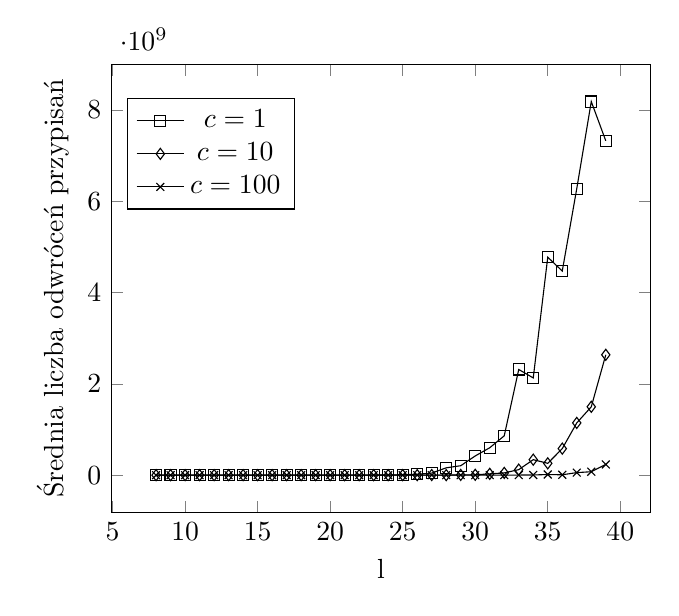
\begin{tikzpicture}
    \begin{axis}[ylabel={Średnia liczba odwróceń przypisań}, xlabel={l}, legend style={at={(0.03,0.8)}, anchor=west}]
    \addplot[
    color=black,
    mark=square,
    ]
    coordinates {
        (8,55.3)(9,241)(10,195.3)(11,815.2)(12,1180.4)(13,1126.7)(14,10774.9)(15,15598.3)(16,23985.7)(17,59097.7)(18,123467.2)(19,277844.4)(20,132090.9)(21,836015.4)(22,1633597.1)(23,2724227.2)(24,3209904.9)(25,10501416.2)(26,18868058.3)(27,45758955.1)(28,160875721.1)(29,207022644.2)(30,420744738.1)(31,600558021.1)(32,861337050.4)(33,2314713706)(34,2129353277)(35,4774140223)(36,4469157089)(37,6275585955)(38,8181380127)(39,7321977601)

    };
    \addlegendentry{$c = 1$}
    \addplot[
    color=black,
    mark=diamond,
    ]
    coordinates {
(8,2)(9,6)(10,11)(11,7)(12,88)(13,71)(14,264)(15,361)(16,936)(17,3559)(18,4443)(19,8583)(20,4456)(21,11667)(22,48127)(23,108675)(24,245824)(25,803191)(26,637552)(27,2266769)(28,1265776)(29,5450840)(30,7557746)(31,28871696)(32,49238112)(33,121225411)(34,338874771)(35,259426141)(36,580907270)(37,1144204637)(38,1496673416)(39,2635124524)

    };
    \addlegendentry{$c = 10$}
    \addplot[
    color=black,
    mark=x,
    ]
    coordinates{
(8,1)(9,1)(10,2)(11,4)(12,4)(13,10)(14,15)(15,20)(16,43)(17,81)(18,212)(19,278)(20,430)(21,1169)(22,2189)(23,4950)(24,16666)(25,19519)(26,34515)(27,109132)(28,177298)(29,256536)(30,333894)(31,1188660)(32,2259196)(33,2063163)(34,4306589)(35,14044363)(36,8204427)(37,55924970)(38,75371771)(39,234689971)
        
    };
    \addlegendentry{$c = 100$}
    \end{axis}
    \end{tikzpicture}
    \caption{Zależność liczby odwróceń przypisań wykonanych przez solwer WalkSAT od długości ciągu i ilości rekordów dla $NDB$ wygenerowanej za pomocą algorytmu prefiksowego.}
    \label{chrt:prefix-flips}
\end{figure}

\begin{figure}[!htb]
    \centering
    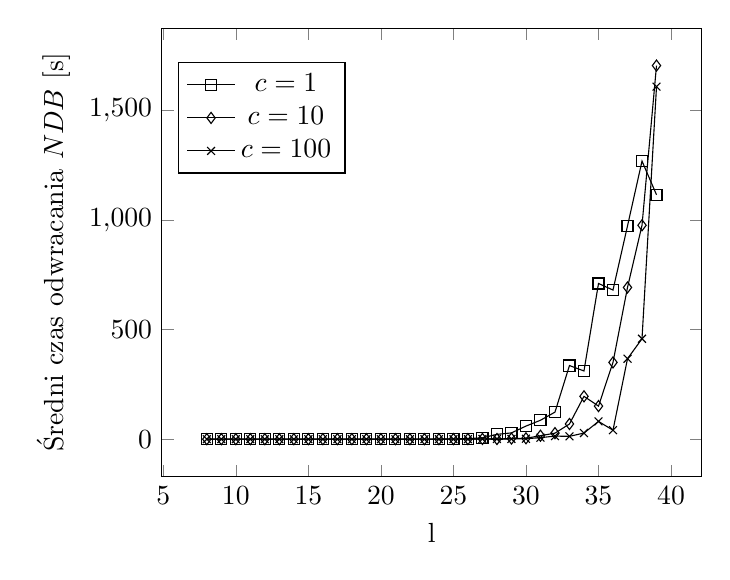
\begin{tikzpicture}
    \begin{axis}[ylabel={Średni czas odwracania $NDB$ [s]}, xlabel={l}, legend style={at={(0.03,0.8)}, anchor=west}]
    \addplot[
    color=black,
    mark=square,
    ]
    coordinates {
        (8,0.00)(9,0.00)(10,0.00)(11,0.00)(12,0.00)(13,0.00)(14,0.00)(15,0.00)(16,0.00)(17,0.01)(18,0.02)(19,0.03)(20,0.02)(21,0.11)(22,0.21)(23,0.36)(24,0.43)(25,1.42)(26,2.58)(27,6.30)(28,22.04)(29,28.64)(30,59.78)(31,86.30)(32,123.38)(33,335.89)(34,311.03)(35,710.14)(36,680.19)(37,972.53)(38,1268.39)(39,1114.68)
        
    };
    \addlegendentry{$c = 1$}
    \addplot[
    color=black,
    mark=diamond,
    ]
    coordinates {
        (8,0)(9,0)(10,0)(11,0)(12,0)(13,0)(14,0)(15,0)(16,0.0003)(17,0.0013)(18,0.0016)(19,0.0036)(20,0.0018)(21,0.0051)(22,0.0216)(23,0.0498)(24,0.1148)(25,0.388)(26,0.3231)(27,1.1604)(28,0.6626)(29,2.8927)(30,4.1046)(31,15.9142)(32,27.5103)(33,69.3003)(34,195.4289)(35,150.9238)(36,350.2829)(37,692.0169)(38,975.5815)(39,1703.9504)
        
    };
    \addlegendentry{$c = 10$}
    \addplot[
    color=black,
    mark=x,
    ]
    coordinates{
        (8,0)(9,0)(10,0)(11,0)(12,0)(13,0)(14,0)(15,0)(16,0)(17,0)(18,0)(19,0)(20,0)(21,0)(22,0)(23,0)(24,0)(25,0)(26,0)(27,1)(28,1)(29,1)(30,2)(31,7)(32,14)(33,13)(34,28)(35,81)(36,41)(37,367)(38,458)(39,1608)


        
    };
    \addlegendentry{$c = 100$}
    \end{axis}
    \end{tikzpicture}
    \caption{Zależność czasu koniecznego do znalezienia pierwszego rozwiązania przez solwer WalkSAT od długości ciągu i ilości rekordów dla $NDB$ wygenerowanej za pomocą algorytmu prefiksowego.}
    \label{chrt:prefix-time-w}
\end{figure}


%%%%%%%%%%%%%%%%%%%%%%%%%%%%%%%%%%%%%%%%%%%%%%%%%%%%%%%%%%%%%%%%%%%%%%%%%%%%%%%%%%%%%%%%%%%%%%%%%%%%%%%%%%%%%%%%%%%%%%%%%%%%%%%%%%%%%%%%%%%%%%%%%%%%%%%%%%%%%%%%%%%%%%%%%%%%%%%%%%%%%%%%%%%%%%%%%%%%%%%%%%%%%%%%%%%%%%%%%%%%%%%%%%%%
\subsection{Algorytm \textit{Randomize\_NDB}}
%%%%%%%%%%%%%%%%%%%%%%%%%%%%%%%%%%%%%%%%%%%%%%%%%%%%%%%%%%%%%%%%%%%%%%%%%%%%%%%%%%%%%%%%%%%%%%%%%%%%%%%%%%%%%%%%%%%%%%%%%%%%%%%%%%%%%%%%%%%%%%%%%%%%%%%%%%%%%%%%%%%%%%%%%%%%%%%%%%%%%%%%%%%%%%%%%%%%%%%%%%%%%%%%%%%%%%%%%%%%%%%%%%%%

Algorytm \textit{Randomize\_NDB} generuje bazy danych o znacznie większym rozmiarze niż algorytm prefiksowy. Już dla 25 rekordów, każdy o długości co najmniej 300 bitów, czas trwania procedury generacyjnej przekracza godzinę,
podczas, gdy czas rozwiązywania bazy o takich parametrach zajmuje solwerowi zChaff niecałe dwie sekundy. Dla ukrywania pojedynczych rekordów procedura działa niewiele wolniej niż algorytm prefiksowy, ale wynikowa $NDB$ będzie bardzo prosta do złamania.

Złożoność otrzymanej bazy zależy głównie od ilości zawartych rekordów pozytywnych, ale czas generacji rośnie dużo szybciej niż trudność problemu SAT. z wykresu \ref{chrt:rand-time-z} na pierwszy rzut oka wynika, że dla większych wartości $l$ czas rozwiązania znacznie wzrasta, ale jest to spowodowane
procesem przetwarzania wstępnego solwera zChaff -- dla wszystkich pokazanych przykładów liczba podjętych decyzji nie przekracza pięciu.

Solwer WalkSAT podobnie jak w przypadku algorytmu prefiksowego wypada znacznie gorzej niż zChaff, jednak tym razem potrafi w krótkim czasie odwrócić $NDB$ przy $l=100$ i niewielkiej ilości rekordów pozytywnych, jednak wraz ze wzrostem $c$ złożoność obliczeniowa zwiększa się drastycznie.

\begin{figure}[!h]
    \centering
    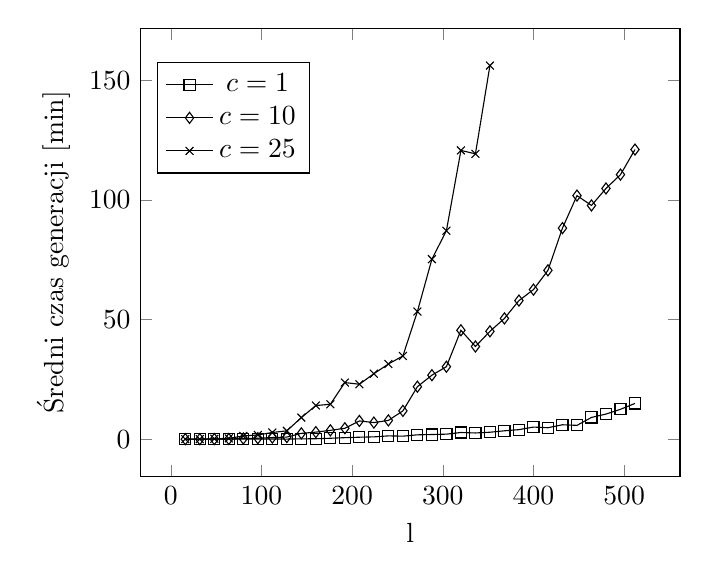
\begin{tikzpicture}
    \begin{axis}[ylabel={Średni czas generacji [min]}, xlabel={l}, legend style={at={(0.03,0.8)}, anchor=west}]
    \addplot[
    color=black,
    mark=square,
    ]
    coordinates {
        (16,0.00025)(32,0.00115)(48,0.003733333333)(64,0.004266666667)(80,0.02518333333)(96,0.05383333333)(112,0.09065)(128,0.04515)(144,0.1289833333)(160,0.1882666667)(176,0.3859666667)(192,0.6316166667)(208,0.82445)(224,0.96245)(240,1.374933333)(256,1.260816667)(272,1.815816667)(288,1.946533333)(304,2.09925)(320,2.791583333)(336,2.594833333)(352,2.902866667)(368,3.498683333)(384,3.981716667)(400,5.058816667)(416,4.78275)(432,6.022966667)(448,5.771866667)(464,9.091316667)(480,10.48951667)(496,12.47911667)(512,14.94341667)

    };
    \addlegendentry{$c = 1$}
    \addplot[
    color=black,
    mark=diamond,
    ]
    coordinates {
        (16,0.00085)(32,0.008866666667)(48,0.04466666667)(64,0.08683333333)(80,0.2802333333)(96,0.4084666667)(112,0.6871833333)(128,0.87305)(144,2.4365)(160,2.942483333)(176,3.691433333)(192,4.55565)(208,7.617466667)(224,6.938716667)(240,7.843183333)(256,11.82141667)(272,21.93571667)(288,26.74303333)(304,30.27935)(320,45.50025)(336,38.72085)(352,45.04981667)(368,50.45198333)(384,57.90636667)(400,62.48886667)(416,70.54368333)(432,88.1753)(448,101.7783333)(464,97.65956667)(480,104.7520167)(496,110.5336667)(512,121.0154167)

    };
    \addlegendentry{$c = 10$}
    \addplot[
    color=black,
    mark=x,
    ]
    coordinates{
        (16,0.003966666667)(32,0.03453333333)(48,0.1718333333)(64,0.3356)(80,1.350816667)(96,1.759766667)(112,2.79695)(128,3.484116667)(144,9.031316667)(160,14.05761667)(176,14.58041667)(192,23.65731667)(208,22.94568333)(224,27.3603)(240,31.40791667)(256,34.77282667)(272,53.32652714)(288,75.21356095)(304,87.10059476)(320,120.6542952)(336,119.2079957)(352,156.0950167)
    };
    \addlegendentry{$c = 25$}
    \end{axis}
    \end{tikzpicture}
    \caption{Zależność czasu generacji $NDB$ za pomocą algorytmu \textit{Randomize\_NDB} od długości kodowanego ciągu.}
    \label{chrt:rand-timegen}
\end{figure}

\begin{figure}[!h]
    \centering
    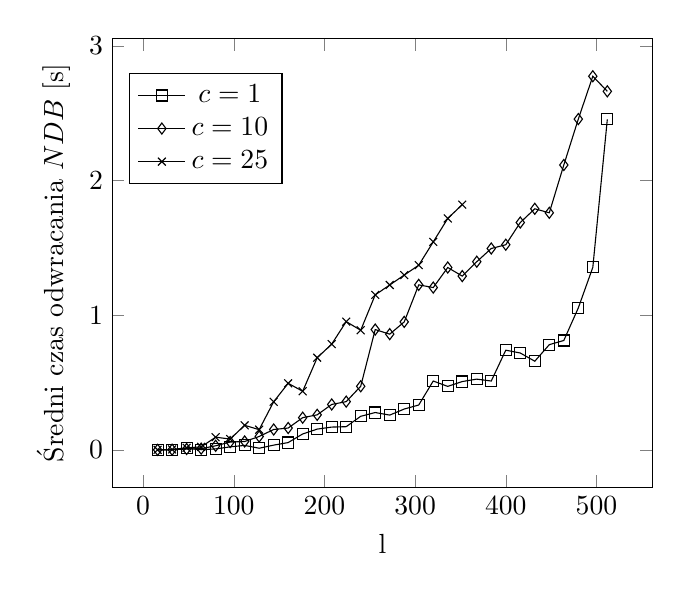
\begin{tikzpicture}
    \begin{axis}[ylabel={Średni czas odwracania $NDB$ [s]}, xlabel={l}, legend style={at={(0.03,0.8)}, anchor=west}]
    \addplot[
    color=black,
    mark=square,
    ]
    coordinates {
(16,0)(32,0)(48,0.012)(64,0.001)(80,0.007)(96,0.022)(112,0.033)(128,0.012)(144,0.035)(160,0.054)(176,0.118)(192,0.154)(208,0.169)(224,0.172)(240,0.249)(256,0.277)(272,0.258)(288,0.303)(304,0.333)(320,0.511)(336,0.471)(352,0.507)(368,0.525)(384,0.511)(400,0.74)(416,0.719)(432,0.658)(448,0.781)(464,0.812)(480,1.054)(496,1.355)(512,2.454)
    };
    \addlegendentry{$c = 1$}
    \addplot[
    color=black,
    mark=diamond,
    ]
    coordinates {
(16,0)(32,0.001)(48,0.006)(64,0.009)(80,0.03)(96,0.058)(112,0.062)(128,0.099)(144,0.151)(160,0.162)(176,0.239)(192,0.26)(208,0.337)(224,0.358)(240,0.472)(256,0.893)(272,0.859)(288,0.95)(304,1.225)(320,1.205)(336,1.354)(352,1.29)(368,1.397)(384,1.495)(400,1.523)(416,1.688)(432,1.79)(448,1.76)(464,2.115)(480,2.456)(496,2.774)(512,2.662)

    };
    \addlegendentry{$c = 10$}
    \addplot[
    color=black,
    mark=x,
    ]
    coordinates{
(16,0)(32,0.003)(48,0.015)(64,0.022)(80,0.094)(96,0.08)(112,0.182)(128,0.15)(144,0.357)(160,0.494)(176,0.435)(192,0.684)(208,0.785)(224,0.952)(240,0.888)(256,1.150571429)(272,1.224107143)(288,1.297642857)(304,1.371178571)(320,1.544)(336,1.718)(352,1.821)


    };
    \addlegendentry{$c = 25$}
    \end{axis}
    \end{tikzpicture}
    \caption{Zależność czasu koniecznego do znalezienia pierwszego rozwiązania przez solwer zChaff od długości ciągu i ilości rekordów dla $NDB$ wygenerowanej za pomocą algorytmu \textit{Randomize\_NDB}.}
    \label{chrt:rand-time-z}
\end{figure}

\begin{figure}[!h]
    \centering
    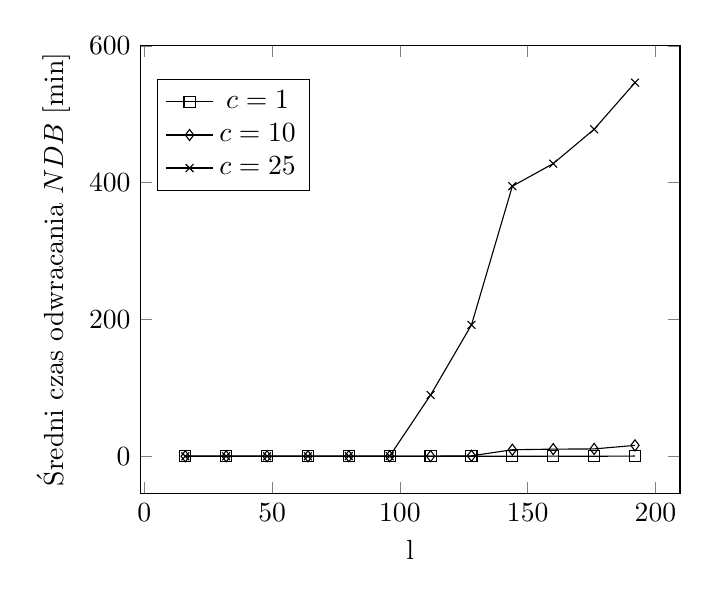
\begin{tikzpicture}
    \begin{axis}[ylabel={Średni czas odwracania $NDB$ [min]}, xlabel={l}, legend style={at={(0.03,0.8)}, anchor=west}]
    \addplot[
    color=black,
    mark=square,
    ]
    coordinates {
        (16,0)(32,0.0001)(48,0.001383333333)(64,0.003033333333)(80,0.0019)(96,0.002583333333)(112,0.00415)(128,0.01401666667)(144,0.02035)(160,0.15425)(176,0.01788333333)(192,0.3611333333)
    };
    \addlegendentry{$c = 1$}
    \addplot[
    color=black,
    mark=diamond,
    ]
    coordinates {
        (16,0.0001)(32,0.0009333333333)(48,0.004516666667)(64,0.01353333333)(80,0.03076666667)(96,0.09353333333)(112,0.23255)(128,0.6885666667)(144,9.571016667)(160,10.45456667)(176,10.78288333)(192,15.94611667)
        
    };
    \addlegendentry{$c = 10$}
    \addplot[
    color=black,
    mark=x,
    ]
    coordinates{
(16,0.0002333333333)(32,0.002333333333)(48,0.02768333333)(64,0.02563333333)(80,0.27615)(96,0.2521333333)(112,89.5563)(128,192.00955)(144,394.8113167)(160,427.7977833)(176,477.9779667)(192,546.0952833)
    };
    \addlegendentry{$c = 25$}
    \end{axis}
    \end{tikzpicture}
    \caption{Zależność czasu koniecznego do znalezienia pierwszego rozwiązania przez solwer WalkSAT od długości ciągu i ilości rekordów dla $NDB$ wygenerowanej za pomocą algorytmu \textit{Randomize\_NDB}.}
    \label{chrt:rand-time-w}
\end{figure}

\begin{figure}[!h]
    \centering
    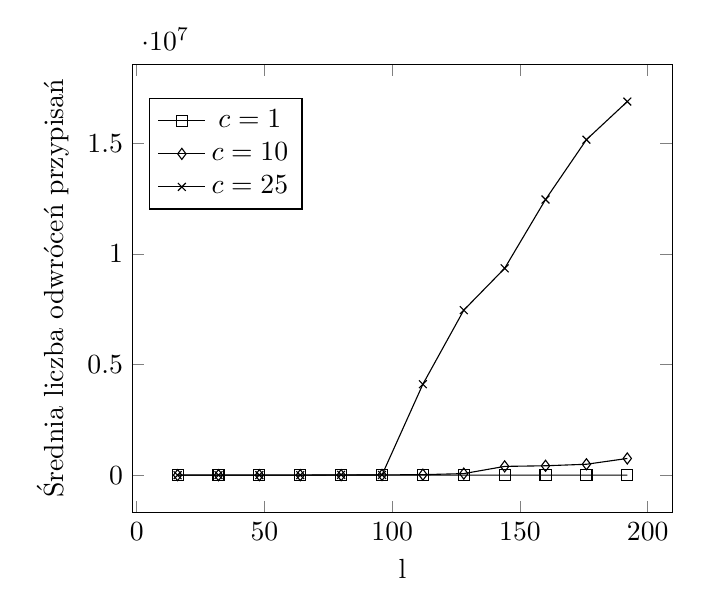
\begin{tikzpicture}
    \begin{axis}[ylabel={Średnia liczba odwróceń przypisań}, xlabel={l}, legend style={at={(0.03,0.8)}, anchor=west}]
    \addplot[
    color=black,
    mark=square,
    ]
    coordinates {
(16,25)(32,17)(48,85)(64,250)(80,384)(96,87)(112,486)(128,1317)(144,1862)(160,528)(176,293)(192,2640)
    };
    \addlegendentry{$c = 1$}
    \addplot[
    color=black,
    mark=diamond,
    ]
    coordinates {
(16,12)(32,166)(48,608)(64,514)(80,735)(96,10632)(112,22201)(128,69959)(144,395594)(160,423950)(176,492287)(192,754665)
        
    };
    \addlegendentry{$c = 10$}
    \addplot[
    color=black,
    mark=x,
    ]
    coordinates{
        (16,5)(32,227)(48,2458)(64,559)(80,14469)(96,9295)(112,4110095)(128,7454363)(144,9345394)(160,12454067)(176,15157587)(192,16879978)
    };
    \addlegendentry{$c = 25$}
    \end{axis}
    \end{tikzpicture}
    \caption{Zależność liczby odwróceń przypisań wykonanych przez solwer WalkSAT od długości ciągu i ilości rekordów dla $NDB$ wygenerowanej za pomocą algorytmu \textit{Randomize\_NDB}.}
    \label{chrt:rand-flips}
\end{figure}

\pagebreak
~~~
\pagebreak

%%%%%%%%%%%%%%%%%%%%%%%%%%%%%%%%%%%%%%%%%%%%%%%%%%%%%%%%%%%%%%%%%%%%%%%%%%%%%%%%%%%%%%%%%%%%%%%%%%%%%%%%%%%%%%%%%%%%%%%%%%%%%%%%%%%%%%%%%%%%%%%%%%%%%%%%%%%%%%%%%%%%%%%%%%%%%%%%%%%%%%%%%%%%%%%%%%%%%%%%%%%%%%%%%%%%%%%%%%%%%%%%%%%%
\subsection{Algorytm \textit{Q-Hidden}}
%%%%%%%%%%%%%%%%%%%%%%%%%%%%%%%%%%%%%%%%%%%%%%%%%%%%%%%%%%%%%%%%%%%%%%%%%%%%%%%%%%%%%%%%%%%%%%%%%%%%%%%%%%%%%%%%%%%%%%%%%%%%%%%%%%%%%%%%%%%%%%%%%%%%%%%%%%%%%%%%%%%%%%%%%%%%%%%%%%%%%%%%%%%%%%%%%%%%%%%%%%%%%%%%%%%%%%%%%%%%%%%%%%%%
W przeciwieństwie do poprzednich algorytmów, \textit{Q-Hidden} generuje $NDB$, które mogą przechowywać jedynie jeden rekord pozytywny. Nie jest to jednak problemem dla systemów przechowujących znaczne ilości danych, gdyż
pomimo konieczności tworzenia osobnej bazy dla każdego rekordu, takie podejście zapewnia dużo krótsze czasy generacji i dużo mniej potrzebnej przestrzeni dyskowej niż algorytmy prefiksowy i \textit{Randomize\_NDB}.
Znacznie zredukowanie liczby rekordów negatywnych powoduje też skrócenie czasu zapytań.

\begin{figure}[!htb]
    \centering
    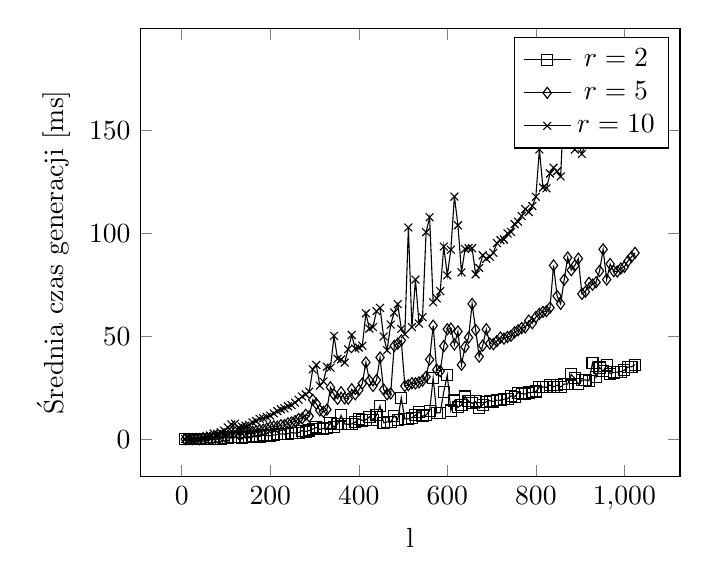
\begin{tikzpicture}
    \begin{axis}[ylabel={Średnia czas generacji [ms]}, xlabel={l}]
    \addplot[
    color=black,
    mark=square,
    ]
    coordinates {
        (8,0)(16,0)(24,0)(32,0)(40,0)(48,0.02)(56,0.02)(64,0.06)(72,0.06)(80,0.02)(88,0.12)(96,0.76)(104,0.6)(112,1.04)(120,1.18)(128,1.06)(136,0.62)(144,0.96)(152,1.2)(160,1.42)(168,1.56)(176,1.34)(184,2.08)(192,1.72)(200,1.68)(208,2)(216,2.32)(224,2.56)(232,2.5)(240,2.7)(248,3.14)(256,3)(264,3.18)(272,4.08)(280,3.7)(288,4.22)(296,4.94)(304,5.7)(312,4.84)(320,5.18)(328,5.26)(336,7.66)(344,5.9)(352,7.34)(360,11.54)(368,7.42)(376,7.22)(384,7.42)(392,8.2)(400,9.86)(408,9.12)(416,9.36)(424,10.9)(432,9.52)(440,11.62)(448,16.2)(456,7.96)(464,8.4)(472,8.24)(480,11.42)(488,9.4)(496,20.18)(504,9.82)(512,9.98)(520,10.46)(528,11.66)(536,13.28)(544,11.08)(552,11.78)(560,13.76)(568,29.72)(576,12.72)(584,12.9)(592,23.08)(600,31.16)(608,13.9)(616,18.76)(624,15.44)(632,16.6)(640,20.72)(648,18.54)(656,17.46)(664,18.34)(672,14.98)(680,16.78)(688,18.24)(696,18.74)(704,18.34)(712,18.96)(720,18.94)(728,19.42)(736,19.7)(744,21.04)(752,20.62)(760,22.64)(768,22.16)(776,21.9)(784,22.66)(792,22.76)(800,23.18)(808,25.26)(816,25.36)(824,25.22)(832,26.3)(840,25.46)(848,26.2)(856,25.38)(864,26.84)(872,26.74)(880,31.46)(888,29.54)(896,26.76)(904,28.74)(912,28.78)(920,28.44)(928,36.98)(936,30.08)(944,34.82)(952,33.14)(960,35.84)(968,31.78)(976,32.44)(984,32.62)(992,32.84)(1000,33.5)(1008,35.08)(1016,35.16)(1024,36.18)
    };
    \addlegendentry{$r = 2$}
    \addplot[
    color=black,
    mark=diamond,
    ]
    coordinates {
        (8,0)(16,0)(24,0.02)(32,0.1)(40,0)(48,0.16)(56,0.52)(64,0.46)(72,0.74)(80,0.82)(88,1.28)(96,1.5)(104,1.7)(112,3.3)(120,3.38)(128,2.72)(136,2.74)(144,3.38)(152,3.28)(160,3.68)(168,3.84)(176,4.34)(184,4.6)(192,5.2)(200,5.82)(208,6.22)(216,6.08)(224,6.8)(232,6.88)(240,7.72)(248,8.14)(256,8.78)(264,9.78)(272,10.12)(280,11.84)(288,11.1)(296,19.12)(304,17.26)(312,14)(320,13.32)(328,14.4)(336,25.18)(344,21.66)(352,19.64)(360,22.82)(368,19.8)(376,19.7)(384,24.26)(392,21.84)(400,23.86)(408,27.06)(416,37.32)(424,28.48)(432,25.86)(440,28.68)(448,39.7)(456,24.14)(464,21.82)(472,22.22)(480,45.36)(488,46.44)(496,48)(504,25.84)(512,26.3)(520,27.22)(528,27.1)(536,27.64)(544,28.46)(552,30.3)(560,38.74)(568,55.2)(576,33.72)(584,33.1)(592,45.22)(600,53.42)(608,53.76)(616,46.02)(624,52.36)(632,36.16)(640,44.84)(648,49.4)(656,65.76)(664,53.1)(672,40.14)(680,45.5)(688,53.4)(696,46.46)(704,46.18)(712,47.68)(720,49.38)(728,48.88)(736,49.66)(744,50.28)(752,51.96)(760,52.94)(768,54)(776,54.32)(784,57.6)(792,56.38)(800,59.34)(808,60.92)(816,61.84)(824,62.22)(832,63.92)(840,84.46)(848,69.58)(856,65.78)(864,77.5)(872,88.3)(880,82.14)(888,84.38)(896,87.74)(904,70.62)(912,71.64)(920,75.96)(928,75.1)(936,76.28)(944,81.8)(952,92.26)(960,77.58)(968,85.14)(976,81.66)(984,81.52)(992,82.96)(1000,83.78)(1008,86.54)(1016,88.62)(1024,90.52)
    };
    \addlegendentry{$r = 5$}
    \addplot[
    color=black,
    mark=x,
    ]
    coordinates{
        (8,0)(16,0.02)(24,0.08)(32,0.38)(40,0.72)(48,0.88)(56,1.46)(64,1.78)(72,2.7)(80,2.58)(88,3.34)(96,4.18)(104,5.7)(112,7.18)(120,7.48)(128,5.5)(136,6.14)(144,6.56)(152,6.94)(160,8.14)(168,8.78)(176,9.96)(184,10.16)(192,10.84)(200,11.44)(208,12.52)(216,13.64)(224,14.48)(232,15)(240,16.02)(248,16.52)(256,17.78)(264,19.16)(272,20.74)(280,21.74)(288,23.14)(296,33.94)(304,36.08)(312,25.98)(320,28.06)(328,35.2)(336,34.76)(344,50.18)(352,39.06)(360,38.76)(368,37.22)(376,43.72)(384,50.64)(392,44.04)(400,44.54)(408,45.42)(416,61.16)(424,53.74)(432,54.48)(440,62.22)(448,63.8)(456,49.88)(464,43.26)(472,55.68)(480,61.56)(488,65.64)(496,53.6)(504,50.98)(512,102.9)(520,54.48)(528,77.58)(536,56.2)(544,59.3)(552,100.62)(560,107.86)(568,66.56)(576,68.46)(584,71.92)(592,93.58)(600,79.62)(608,92.1)(616,117.9)(624,103.96)(632,81.04)(640,92.44)(648,92.86)(656,92.84)(664,80.1)(672,83.24)(680,89.4)(688,87.7)(696,88.68)(704,90.64)(712,95.3)(720,96.7)(728,97.06)(736,99.98)(744,100.74)(752,104.52)(760,105.68)(768,108.48)(776,111.84)(784,110.42)(792,113.3)(800,117.82)(808,140.78)(816,122.3)(824,121.92)(832,129.12)(840,131.94)(848,130.26)(856,127.7)(864,165.54)(872,178.44)(880,146.08)(888,140.76)(896,144.42)(904,138.6)(912,143.48)(920,154.32)(928,148.58)(936,157.38)(944,178.94)(952,155.52)(960,160.9)(968,161.96)(976,162.6)(984,164.18)(992,167.86)(1000,170.44)(1008,175.2)(1016,174.22)(1024,181.58)
        
       
    };
    \addlegendentry{$r = 10$}
    \end{axis}
    \end{tikzpicture}
    \caption{Zależność czasu generacji $NDB$ za pomocą algorytmu \textit{Q-Hidden} od długości kodowanego ciągu.}
    \label{chrt:q-gen}
\end{figure}

Algorytm \textit{Q-Hidden} tworzy bazy o dowolnie konfigurowanej, stałej liczbie rekordów. Generacja $NDB$ jest bardzo szybka i dokonuje się w czasie liniowym od iloczynu parametrów $r$ oraz $l$.


\begin{figure}[!htb]
    \centering
    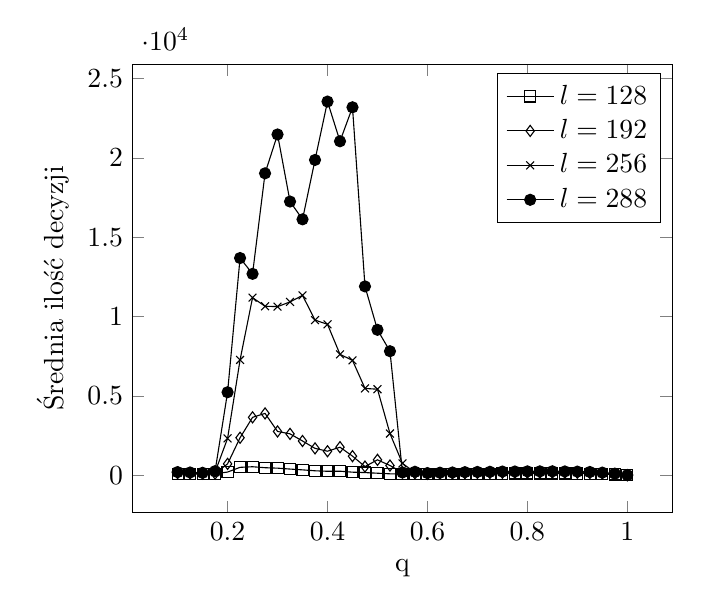
\begin{tikzpicture}
    \begin{axis}[ylabel={Średnia ilość decyzji}, xlabel={q}]
    \addplot[
    color=black,
    mark=square,
    ]
    coordinates {
        (0.1,87.68686869)(0.125,80.41)(0.15,67.41)(0.175,89.57)(0.2,196.92)(0.225,493.57)(0.25,531.31)(0.275,470.12)(0.3,441.73)(0.325,384.67)(0.35,334.25)(0.375,276.07)(0.4,244.87)(0.425,249.96)(0.45,189)(0.475,163.09)(0.5,123.32)(0.525,85.39)(0.55,66.83)(0.575,63.21)(0.6,66.73)(0.625,70.62)(0.65,77.02)(0.675,83.98)(0.7,90.39)(0.725,95.04)(0.75,99.97)(0.775,104.21)(0.8,105.96)(0.825,108.07)(0.85,107.24)(0.875,105.75)(0.9,100.32)(0.925,89.85)(0.95,71.95)(0.975,43.81)(1,1)
    };
    \addlegendentry{$l = 128$}
    \addplot[
    color=black,
    mark=diamond,
    ]
    coordinates {
        (0.1,129.25)(0.125,114.75)(0.15,100.35)(0.175,101.9)(0.2,712.55)(0.225,2357.1)(0.25,3644.4)(0.275,3892.8)(0.3,2756.05)(0.325,2602.95)(0.35,2153.9)(0.375,1689.65)(0.4,1508.75)(0.425,1763.25)(0.45,1199.7)(0.475,543.3)(0.5,966.2)(0.525,609)(0.55,168.45)(0.575,116.6)(0.6,82.35)(0.625,102.85)(0.65,112.1)(0.675,123.8)(0.7,140)(0.725,141.65)(0.75,148.5)(0.775,155.9)(0.8,159.9)(0.825,159.8)(0.85,161.65)(0.875,156.6)(0.9,150.5)(0.925,134.05)(0.95,109)(0.975,63.15)(1,0.9523809524)
    };
    \addlegendentry{$l = 192$}
    \addplot[
    color=black,
    mark=x,
    ]
    coordinates{
    
        (0.1,172.11)(0.125,150.59)(0.15,125.95)(0.175,193.52)(0.2,2318.1)(0.225,7263.85)(0.25,11187.44)(0.275,10646.52)(0.3,10621.72)(0.325,10919.14)(0.35,11329.77)(0.375,9775.06)(0.4,9506.85)(0.425,7613.82)(0.45,7236)(0.475,5465.65)(0.5,5417.52)(0.525,2625.65)(0.55,741.15)(0.575,171.64)(0.6,135.47)(0.625,137.16)(0.65,154.28)(0.675,166.99)(0.7,180.42)(0.725,188.23)(0.75,198.9)(0.775,206.28)(0.8,212.15)(0.825,214.92)(0.85,214.06)(0.875,210.9)(0.9,199.13)(0.925,176.7)(0.95,143.06)(0.975,86.65)(1,1)
        
    };
    \addlegendentry{$l = 256$}
        \addplot[
    color=black,
    mark=*,
    ]
    coordinates{
        (0.1,193.35)(0.125,169.9)(0.15,148.95)(0.175,252.5)(0.2,5226.45)(0.225,13685)(0.25,12688.05)(0.275,19023.2)(0.3,21472.3)(0.325,17244.85)(0.35,16123.45)(0.375,19865.75)(0.4,23545.65)(0.425,21043.5)(0.45,23185.15)(0.475,11896.8)(0.5,9160.65)(0.525,7811.35)(0.55,170.15)(0.575,212.75)(0.6,132.95)(0.625,156.85)(0.65,169)(0.675,189.55)(0.7,203.65)(0.725,212.25)(0.75,226.75)(0.775,230.6)(0.8,239.05)(0.825,239.25)(0.85,243.7)(0.875,233.95)(0.9,223.55)(0.925,201.25)(0.95,160.25)(0.975,96.3)(1,1)
    };
    \addlegendentry{$l = 288$}
    \end{axis}
    \end{tikzpicture}
    \caption{Zależność liczby decyzji potrzebnych do znalezienia pierwszego rozwiązania przez solwer zChaff od parametru $q$ dla $NDB$ wygenerowanej za pomocą algorytmu \textit{Q-Hidden} przy parametrach $r=5.5$ i $k=3$.}
    \label{chrt:q-q-z}
\end{figure}


\begin{figure}[!htb]
    \centering
    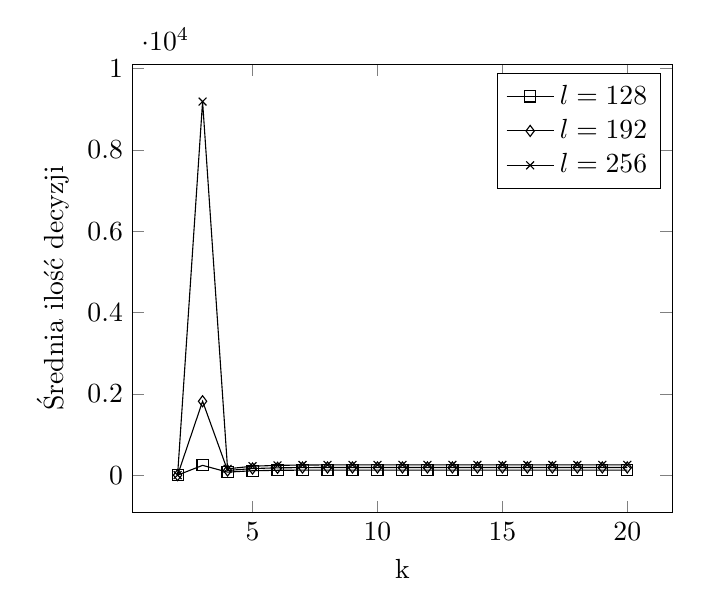
\begin{tikzpicture}
    \begin{axis}[ylabel={Średnia ilość decyzji}, xlabel={k}]
    \addplot[
    color=black,
    mark=square,
    ]
    coordinates {
(2,4.1)(3,244.5)(4,78.06666667)(5,112.2333333)(6,123.2)(7,126.8)(8,127.9666667)(9,128.6666667)(10,128.7)(11,128.9666667)(12,129)(13,128.9666667)(14,129)(15,129)(16,129)(17,129)(18,129)(19,129)(20,129)
    };
    \addlegendentry{$l = 128$}
    \addplot[
    color=black,
    mark=diamond,
    ]
    coordinates {
(2,4.5)(3,1820.433333)(4,118.8)(5,165.9666667)(6,183.6333333)(7,189.5666667)(8,191.7333333)(9,192.5)(10,192.6666667)(11,192.9666667)(12,192.9333333)(13,193)(14,193)(15,193)(16,193)(17,193)(18,193)(19,193)(20,193)
    };
    \addlegendentry{$l = 192$}
    \addplot[
    color=black,
    mark=x,
    ]
    coordinates{
        
(2,5.6)(3,9188.9)(4,159.4)(5,224.0333333)(6,243.6666667)(7,253.6)(8,255.1666667)(9,256.2666667)(10,256.7333333)(11,256.9333333)(12,256.9)(13,257)(14,257)(15,257)(16,257)(17,257)(18,257)(19,257)(20,257)
        
    };
    \addlegendentry{$l = 256$}
    \end{axis}
    \end{tikzpicture}
    \caption{Zależność liczby decyzji potrzebnych do znalezienia pierwszego rozwiązania przez solwer zChaff od parametru $k$ dla $NDB$ wygenerowanej za pomocą algorytmu \textit{Q-Hidden} przy parametrach $r=5.5$ i $q=0.4$.
        Szczyt zachodzi dla parametru $k=3$.
    }
    \label{chrt:q-k-z}
\end{figure}

\begin{figure}[!htb]
    \centering
    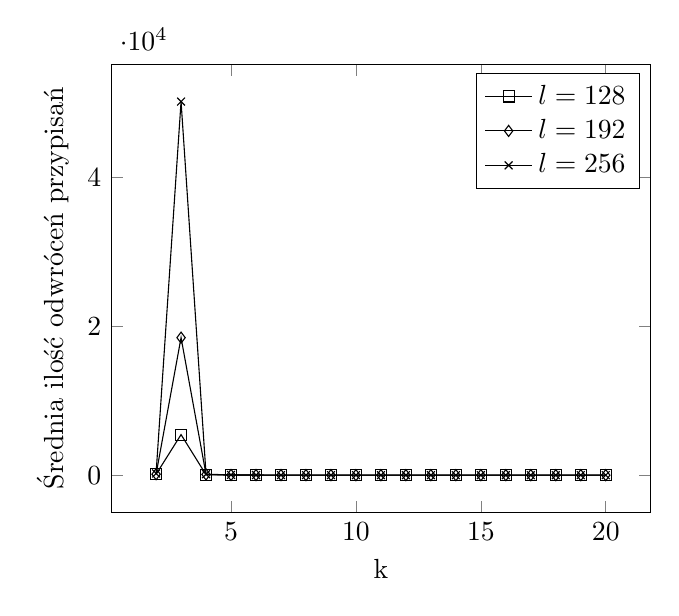
\begin{tikzpicture}
    \begin{axis}[ylabel={Średnia ilość odwróceń przypisań}, xlabel={k}]
    \addplot[
    color=black,
    mark=square,
    ]
    coordinates {
(2,117.2333333)(3,5454.266667)(4,57.6)(5,16.76666667)(6,9.966666667)(7,5)(8,2.466666667)(9,1)(10,0.8)(11,0.3666666667)(12,0.1666666667)(13,0.2)(14,0.1)(15,0.03333333333)(16,0)(17,0)(18,0)(19,0)(20,0)
    };
    \addlegendentry{$l = 128$}
    \addplot[
    color=black,
    mark=diamond,
    ]
    coordinates {
(2,129)(3,18491.23333)(4,93.66666667)(5,25.66666667)(6,13.7)(7,7.233333333)(8,3.4)(9,2.1)(10,0.8333333333)(11,0.4666666667)(12,0.4)(13,0.1333333333)(14,0.1666666667)(15,0)(16,0)(17,0)(18,0)(19,0)(20,0)
    };
    \addlegendentry{$l = 192$}
    \addplot[
    color=black,
    mark=x,
    ]
    coordinates{
        
(2,223.4333333)(3,50237.33333)(4,129.8)(5,31.8)(6,16.8)(7,9.5)(8,5.166666667)(9,2.8)(10,1.333333333)(11,0.8333333333)(12,0.4)(13,0.3)(14,0.1)(15,0.06666666667)(16,0)(17,0)(18,0)(19,0)(20,0)
        
    };
    \addlegendentry{$l = 256$}
    \end{axis}
    \end{tikzpicture}
    \caption{Zależność liczby odwróceń przypisań potrzebnych do znalezienia pierwszego rozwiązania przez solwer WalkSAT od parametru $k$ dla $NDB$ wygenerowanej za pomocą algorytmu \textit{Q-Hidden} przy parametrach $r=5.5$ i $q=0.4$.
        Szczyt zachodzi dla parametru $k=3$.
    }
    \label{chrt:q-k-w}
\end{figure}

\begin{figure}[!htb]
    \centering
    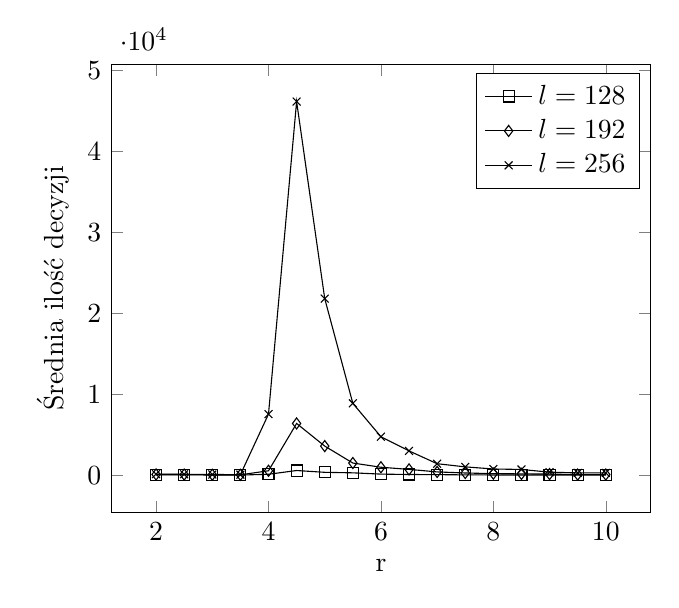
\begin{tikzpicture}
    \begin{axis}[ylabel={Średnia ilość decyzji}, xlabel={r}]
    \addplot[
    color=black,
    mark=square,
    ]
    coordinates {
(2,86)(2.5,77)(3,64)(3.5,54)(4,152)(4.5,614)(5,393)(5.5,329)(6,171)(6.5,122)(7,107)(7.5,77)(8,66)(8.5,59)(9,61)(9.5,45)(10,42)
    };
    \addlegendentry{$l = 128$}
    \addplot[
    color=black,
    mark=diamond,
    ]
    coordinates {
(2,126)(2.5,117)(3,93)(3.5,85)(4,584)(4.5,6419)(5,3629)(5.5,1538)(6,1019)(6.5,754)(7,442)(7.5,309)(8,230)(8.5,202)(9,172)(9.5,114)(10,116)
    };
    \addlegendentry{$l = 192$}
    \addplot[
    color=black,
    mark=x,
    ]
    coordinates{
        
(2,170)(2.5,152)(3,124)(3.5,106)(4,7578)(4.5,46131)(5,21824)(5.5,8901)(6,4782)(6.5,3034)(7,1453)(7.5,1064)(8,803)(8.5,745)(9,410)(9.5,322)(10,320)
        
    };
    \addlegendentry{$l = 256$}
    \end{axis}
    \end{tikzpicture}
    \caption{Zależność liczby decyzji potrzebnych do znalezienia pierwszego rozwiązania przez solwer zChaff od parametru $r$ dla $NDB$ wygenerowanej za pomocą algorytmu \textit{Q-Hidden} przy parametrach $k=3$ i $q=0.4$.}
    \label{chrt:q-r-z}
\end{figure}

\begin{figure}[!htb]
    \centering
    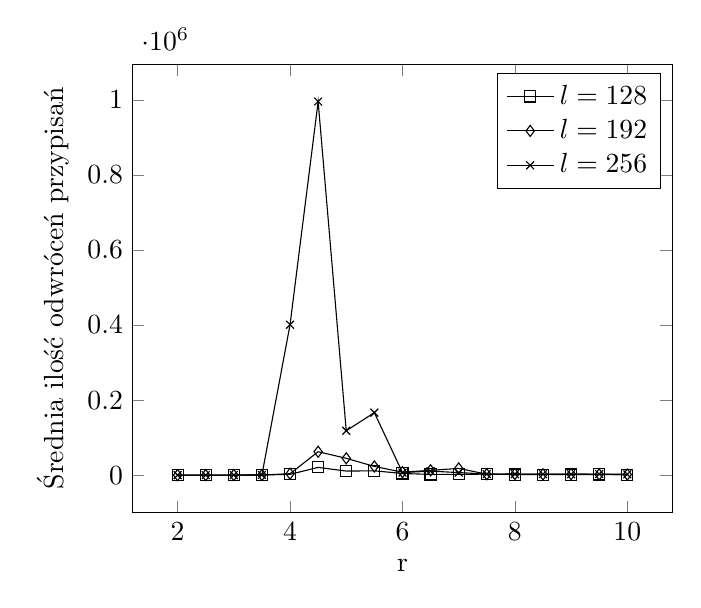
\begin{tikzpicture}
    \begin{axis}[ylabel={Średnia ilość odwróceń przypisań}, xlabel={r}]
    \addplot[
    color=black,
    mark=square,
    ]
    coordinates {
(2,36)(2.5,55)(3,95)(3.5,348)(4,2212)(4.5,20640)(5,10918)(5.5,11528)(6,4471)(6.5,1966)(7,2106)(7.5,2739)(8,1575)(8.5,1317)(9,1644)(9.5,1874)(10,1069)
    };
    \addlegendentry{$l = 128$}
    \addplot[
    color=black,
    mark=diamond,
    ]
    coordinates {
(2,50)(2.5,82)(3,173)(3.5,403)(4,3818)(4.5,62375)(5,44916)(5.5,23211)(6,7983)(6.5,12837)(7,17968)(7.5,2586)(8,3126)(8.5,2208)(9,2711)(9.5,2008)(10,1758)
    };
    \addlegendentry{$l = 192$}
    \addplot[
    color=black,
    mark=x,
    ]
    coordinates{
        
(2,69)(2.5,112)(3,202)(3.5,645)(4,400787)(4.5,995525)(5,118296)(5.5,166596)(6,6763)(6.5,10781)(7,6841)(7.5,2924)(8,2855)(8.5,2581)(9,2372)(9.5,2897)(10,2161)
        
    };
    \addlegendentry{$l = 256$}
    \end{axis}
    \end{tikzpicture}
    \caption{Zależność liczby odwróceń przypisań do znalezienia pierwszego rozwiązania przez solwer WalkSAT od parametru $r$ dla $NDB$ wygenerowanej za pomocą algorytmu \textit{Q-Hidden} przy parametrach $k=3$ i $q=0.4$.}
    \label{chrt:q-r-w}
\end{figure}

%%%%%%%%%%%%%%%%%%%%%%%%%%%%%%%%%%%%%%%%%%%%%%%%%%%%%%%%%%%%%%%%%%%%%%%%%%%%%%%%%%%%%%%%%%%%%%%%%%%%%%%%%%%%%%%%%%%%%%%%%%%%%%%%%%%%%%%%%%%%%%%%%%%%%%%%%%%%%%%%%%%%%%%%%%%%%%%%%%%%%%%%%%%%%%%%%%%%%%%%%%%%%%%%%%%%%%%%%%%%%%%%%%%%
\subsection{Algorytm \textit{K-Hidden}}
%%%%%%%%%%%%%%%%%%%%%%%%%%%%%%%%%%%%%%%%%%%%%%%%%%%%%%%%%%%%%%%%%%%%%%%%%%%%%%%%%%%%%%%%%%%%%%%%%%%%%%%%%%%%%%%%%%%%%%%%%%%%%%%%%%%%%%%%%%%%%%%%%%%%%%%%%%%%%%%%%%%%%%%%%%%%%%%%%%%%%%%%%%%%%%%%%%%%%%%%%%%%%%%%%%%%%%%%%%%%%%%%%%%%


%%%%%%%%%%%%%%%%%%%%%%%%%%%%%%%%%%%%%%%%%%%%%%%%%%%%%%%%%%%%%%%%%%%%%%%%%%%%%%%%%%%%%%%%%%%%%%%%%%%%%%%%%%%%%%%%%%%%%%%%%%%%%%%%%%%%%%%%%%%%%%%%%%%%%%%%%%%%%%%%%%%%%%%%%%%%%%%%%%%%%%%%%%%%%%%%%%%%%%%%%%%%%%%%%%%%%%%%%%%%%%%%%%%%
\subsection{Algorytm hybrydowy}
%%%%%%%%%%%%%%%%%%%%%%%%%%%%%%%%%%%%%%%%%%%%%%%%%%%%%%%%%%%%%%%%%%%%%%%%%%%%%%%%%%%%%%%%%%%%%%%%%%%%%%%%%%%%%%%%%%%%%%%%%%%%%%%%%%%%%%%%%%%%%%%%%%%%%%%%%%%%%%%%%%%%%%%%%%%%%%%%%%%%%%%%%%%%%%%%%%%%%%%%%%%%%%%%%%%%%%%%%%%%%%%%%%%%
